% !TEX encoding = UTF-8 Unicode
\chapter{Sprint 3 - CLI}

\section{Program arguments}
\par
Program is expected 1 to 3 arguments before launching the CLI.
\par
When launching the program the user can give different arguments to the program :
\begin{enumerate}
    \item filePath : simple path to a plain text file path
    \item encrypt filePath password : simple path to a plain text filewhich will be encrypted
    with given password. Output from the CLI will be the path of the cipher file.
    \item cipherFilePath password : path to the cither file, which will be decrypted with the given password.
\end{enumerate}

Based on these different arguments, the main program will handle encryption and decryption
of the file (with FileProcessor class), then send the raw data extracted to the CLI.

\section{CLI}

\begin{figure}[h]
    \begin{center}
        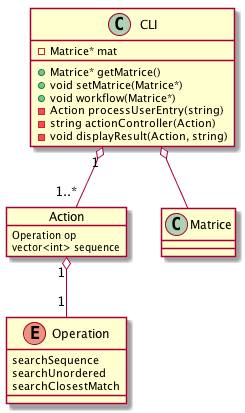
\includegraphics[scale=0.40]{./ressources/graph/CLI.png}
    \end{center}
    \caption{Class diagram}
    \label{Solution - CLI class diagram}
\end{figure}
\bigskip

A simple console log interface (CLI) have been developed in order to enable user to use the pattern research program.\\
Since we don't have to handle a list of operations, the Operation Management class haven't been implemented for simplification of the application.

The CLI is doing the following operations :
\begin{enumerate}
    \item Processing user entry
    \item Calling search operations based on user request and matrice.
    \item Displaying results.
\end{enumerate}
